\documentclass{beamer}%
\usepackage[T1]{fontenc}%
\usepackage[utf8]{inputenc}%
\usepackage{lmodern}%
\usepackage{textcomp}%
\usepackage{lastpage}%
\usepackage{markdown}%
\usepackage[orientation = landscape,size = a3,scale = 1.0]{beamerposter}%
\usepackage{libertine}%
\usepackage[libertine]{newtxmath}%
\usepackage[scaled=.92]{inconsolata}%
%
\usetheme{LLT-poster}%
\usecolortheme{ComingClean}%
\title{PuzzlePalooza}%
\author[info@swissmakers.ch]{Simon Flückiger \textbackslash{}\& Daniel Schmocker}%
\institute{Swiss Makers}%
\footimage{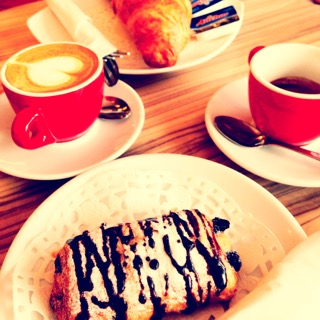
\includegraphics[width=4cm]{IMG_1934.jpg}}%
%
\begin{document}%
\normalsize%
\begin{columns}[T]%
\begin{column}{.32\textwidth}%
\begin{block}{Das Spiel}%
\begin{markdown}
## Die Spielmechanik kurz erklärt

Das Ziel des Spiels ist es, innerhalb einer vorgegebenen Zeit verschiedene Aufgaben zu lösen. Das Spiel wird immer von zwei Personen gespielt, wobei eine Person den "TG 53 Strich 2" bedient und die andere Person die erste Person dazu anleitet. Die erste Person sieht nur den Bildschirm mit dem "TG 53 Strich 2", während die zweite Person nur die Anleitung sieht. Die beiden Personen dürfen nur verbal kommunizieren. Das Spiel ist inspiriert vom Computerspiel "Keep Talking and Nobody Explodes".
![TG53-1](../bilder/TG53-1.jpg)
\end{markdown}%
\end{block}%
\begin{block}{Das Spiel als Projekt}%
\begin{markdown}
## Kollaboratives Making
Unser Projekt stellt ein Spiel dar, für das wir hier unseren ersten Prototypen sowie zwei vereinfachte Varianten präsentieren, die vor allem die Spielmechanik veranschaulichen und zeigen, welche simplen Varianten möglich sind. Alle drei Varianten werden mit der zuvor beschriebenen Spielmechanik gespielt. Sie demonstrieren, was innerhalb einer Projektwoche, eines Projekttags oder -nachmittags mit einer Schulklasse möglich wäre. Wir haben uns aus verschiedenen Gründen für dieses Spiel entschieden: Zum einen arbeiten wir eventorientiert und präsentieren das Spiel zu einem bestimmten Zeitpunkt vor einem ausgewählten Publikum. Zum anderen ist das Spiel modular aufgebaut, sodass die Projektaufgaben je nach Bedarf und Lehrplan modular zusammengestellt werden können, um verschiedene Lerninhalte zu vermitteln.
\end{markdown}%
\end{block}%
\end{column}%
\begin{column}{.32\textwidth}%
\begin{block}{Das Projekt}%
\begin{markdown}
## Warum wir das tun?
Wir entwickeln Maker-Projekte, die als Basis dienen, um mit einer Gruppe in die Welt des Makings einzusteigen. Der Start in diesem Bereich kann oft sehr steinig sein und die Lernkurve sehr steil. Deshalb ist eine gute Begleitung und oft auch eine enge Betreuung notwendig, was mit einem hohen Personalaufwand verbunden sein kann. Unsere Projekte haben immer einen kollaborativen Charakter, sodass Schülerinnen und Schüler gemeinsam an einem Projekt arbeiten.
\end{markdown}%
\end{block}%
\end{column}%
\begin{column}{.32\textwidth}%
\begin{block}{Das Projekt}%
\begin{markdown}
## Warum wir das tun?
Wir entwickeln Maker-Projekte, die als Basis dienen, um mit einer Gruppe in die Welt des Makings einzusteigen. Der Start in diesem Bereich kann oft sehr steinig sein und die Lernkurve sehr steil. Deshalb ist eine gute Begleitung und oft auch eine enge Betreuung notwendig, was mit einem hohen Personalaufwand verbunden sein kann. Unsere Projekte haben immer einen kollaborativen Charakter, sodass Schülerinnen und Schüler gemeinsam an einem Projekt arbeiten.
\end{markdown}%
\end{block}%
\end{column}%
\end{columns}%
\end{document}